\chapter{Ошибки и процессы}
\label{errors-and-processes}
\section{Связи}
\label{links}
Связи \--- это особый вид взаимоотношений, которые могут быть установлены между двумя процессами.
Когда один из процессов, который участвует в таких отношениях, умирает от неожиданного броска, ошибки или завершения (см. \ref{errors-and-exceptions} Ошибки и исключения), то связанный с ним процесс тоже завершается.

Эта концепция может пригодиться, когда требуется как можно быстрее завершить процесс, чтобы предотвратить появление ошибок.
Если процесс, в котором появилась ошибка, завершился аварией, а процессы, которые на него полагаются, продолжили работать, то все эти зависимые процессы должны что\--то предпринять.
Обычно приемлемым вариантом развития событий можно считать остановку и перезапуск всей группы процессов.
Именно это и позволяют нам сделать связи.

Для создания связи между двумя процессами в Erlang существует базовая функция \href{http://erldocs.com/R15B/erts/erlang.html\#link/1}{link/1}, принимающая в качестве аргумента Pid.
После запуска эта функция создаст связь между текущим процессом и процессом, который отождествляется с указанным \emph{Pid}.
Для разрушения связи используют функцию \href{http://erldocs.com/R15B/erts/erlang.html\#unlink/1}{unlink/1}.
При аварийном завершении одного из связанных процессов, отсылается сообщение особого вида, которое несёт информацию относительно произошедших событий.
Если процесс умирает по естественным причинам (читай: завершает исполнение своих функций), то такое сообщение не отсылается.
Для начала поговорим об этой новой функции как об элементе модуля \href{http://learnyousomeerlang.com/static/erlang/linkmon.erl}{linkmon.erl}:
\begin{lstlisting}[style=erlang]
myproc() ->
    timer:sleep(5000),
    exit(reason).
\end{lstlisting}

Если вы попробуете исполнить следущие вызовы функций (и сделаете между каждой командой spawn пятисекундную паузу), то увидите, что оболочка завершится с ошибкой 'reason' только если между двумя процессами была установлена связь.
\begin{lstlisting}[style=erlang]
1> c(linkmon).
{ok,linkmon}
2> spawn(fun linkmon:myproc/0).
<0.52.0>
3> link(spawn(fun linkmon:myproc/0)).
true
** exception error: reason
\end{lstlisting}

Изобразим это на картинке:
\begin{figure}[h!]
    \centering
    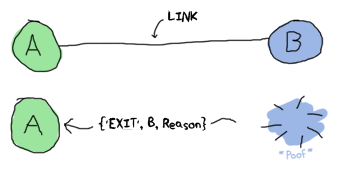
\includegraphics[width=0.7\textwidth]{link-exit.png}
\end{figure}

Для захвата сообщения \ops{\{'EXIT', B, Reason\}} не получится использовать стандартную структуру \ops{try \ldots catch}.
Для этого существуют другие средства, которые мы рассмотрим позже.

Важно отметить, что связи можно также использовать, для организации больших групп процессов, которые должны прекращать исполнения как единая группа, все вместе:
\begin{lstlisting}[style=erlang]
chain(0) ->
    receive
        _ -> ok
    after 2000 ->
        exit("chain dies here")
    end;
chain(N) ->
    Pid = spawn(fun() -> chain(N-1) end),
    link(Pid),
    receive
        _ -> ok
    end.
\end{lstlisting}

Эта функция принимает целое число \emph{N}, запускает \emph{N} связанных между собой процессов.
Для передачи \emph{N-1} аргумента следующему процессу в <<цепи>>, я оборачиваю вызов в анонимную функцию, чтобы она перестала принимать аргументы.
Подобный эффект можно получить при помощи вызова \ops{spawn(?MODULE, chain, [N-1])}.

В этом примере я создам множество связанных процессов, которые будут умирать сразу после завершения их наследников:
\begin{lstlisting}[style=erlang]
4> c(linkmon).              
{ok,linkmon}
5> link(spawn(linkmon, chain, [3])).
true
** exception error: "chain dies here"
\end{lstlisting}

Как видите, оболочка получает сообщение о смерти от одного из процессов.
Вот подробное описание завершения запущенных процессов и уничтожения связей:
\begin{lstlisting}[style=erlang]
[shell] == [3] == [2] == [1] == [0]
[shell] == [3] == [2] == [1] == *dead*
[shell] == [3] == [2] == *dead*
[shell] == [3] == *dead*
[shell] == *dead*
*dead, error message shown*
[shell] <-- restarted
\end{lstlisting}

После завершения процесса, который исполняет функцию \ops{linkmon:chain(0)}, ошибка передаётся по цепи связей, и в результате из\--за неё умирает процесс оболочки.
Авария могла произойти в любом из связанных процессов.
Связи работают в обе стороны, поэтому для завершения всей группы процессов достаточно смерти лишь одного из них.\\
\colorbox{lgray}
{
\begin{minipage}{1.0\linewidth}
    \textbf{Замечание:} если вам необходимо убить из оболочки какой\--либо процесс, то это можно сделать при помощи функции \href{http://erldocs.com/R15B/erts/erlang.html\#exit/2}{exit/2}.
    Её можно вызвать следующим образом: \ops{exit(Pid, Reason)}.
    Можете попробовать ею воспользоваться, если хотите.
\end{minipage}
}
\colorbox{lgray}
{
\begin{minipage}{1.0\linewidth}
    \textbf{Замечание:} связи не накапливаются.
    Если вы вызвали \ops{link/1} 15 раз для одной и той же пары процессов, то между ними будет существовать лишь одна связь, и для её разрушения будет достаточно однократного вызова \ops{unlink/1}.
\end{minipage}
}

Нужно сказать, что вызовы \ops{link(spawn(Function))} или \ops{link(spawn(M,F,A))} совершаются в несколько шагов.
Иногда процесс может умереть до того как была установлена связь, и это спровоцирует неожиданное поведение исполняемого кода.
На такой случай в языке существует функция \href{http://erldocs.com/R15B/erts/erlang.html\#spawn_link/1}{spawn\_link/1-3}.
Она принимает те же самые параметры, что и \ops{spawn/1-3}, создаёт процесс и связывает его, так же как это делает \ops{link/1}, но весь процесс осуществляется атомарной операцией (все действия объединяются в одно, и результатом их исполнения может стать лишь совокупный успех или неудача, никаких других результатов быть не может).
Такой способ создания процессов и их связей считается более надёжным.
К тому же, на нём можно сэкономить пару скобок.
\section{Это ловушка!}
\label{its-a-trap}
\begin{wrapfigure}{r}{0.35\linewidth}
    
\includegraphics[width=1\linewidth]{ackbar.jpg}
\end{wrapfigure}
Вернёмся к связям и умирающим процессам.
Распространение ошибок от процесса к процессу осуществляется методом, похожим на передачу сообщений, но при этом используется их особый тип \--- сигналы.
Сигналы о завершении \--- это <<тайные>> сообщения, которые автоматически действуют на процессы, убивая их во время исполнения.

Я уже неоднократно упоминал, что надёжность приложения зависит от его умения быстро убивать и перезапускать процессы.
На текущий момент в качестве орудия убийства можно использовать связи.
Осталось разобраться с перезапуском.

Чтобы перезапустить процесс, сначала нужно как\--то узнать, что он умер.
Мы можем сделать это, добавив поверх связей ещё один слой (вкусную глазурь на торте), содержащий концепцию, которая называется \emph{системные процессы} (system processes).
Системные процессы, по сути, это обычные процессы, но они могут конвертировать сигналы о завершении в обычные сообщения.
Делают они это при помощи вызова \ops{process\_flag(trap\_exit, true)} в работающем процессе.
Ничто не сможет рассказать об этом механизме больше, чем пример.
Поэтому сейчас мы его и рассмотрим.
Я немного видоизменю пример с chain, поместив в начале системный процесс:
\begin{lstlisting}[style=erlang]
1> process_flag(trap_exit, true).
true
2> spawn_link(fun() -> linkmon:chain(3) end).
<0.49.0>
3> receive X -> X end.
{'EXIT',<0.49.0>,"chain dies here"}
\end{lstlisting}

Ага!
Это уже интереснее.
Вернёмся к нашей иллюстрации.
Теперь картина событий выглядит приблизительно так:
\begin{lstlisting}[style=erlang]
[shell] == [3] == [2] == [1] == [0]
[shell] == [3] == [2] == [1] == *dead*
[shell] == [3] == [2] == *dead*
[shell] == [3] == *dead*
[shell] <-- {'EXIT,Pid,"chain dies here"} -- *dead*
[shell] <-- still alive!
\end{lstlisting}

Вот он, механизм позволяющий быстро перезапускать процессы.
Используя системные процессы при написании программ, можно легко создать процесс, единственная функция которого \--- следить за тем, чтобы все процессы оставались живы, и рестартовать их в случае аварии.
Мы поговорим об этом подробнее в следующей главе, когда будем применять этот приём по\--настоящему.

А сейчас я хочу вернуться к функциям для работы с исключениями, которые мы рассмотрели в главе ~\ref{errors-and-exceptions} об ошибках и исключениях, и увидим как они ведут себя в процессах, которые улавливают факт завершения других процессов.
Сначала  определим основание для эксперимента, не используя системный процесс.
Я последовательно приведу результаты, которые возвращают непойманные броски, ошибки и завершения (exits) в соседних процессах:

\begin{itemize}
    \item \textbf{Источник исключения:} \ops{spawn\_link(fun() -> ok end)}\\
    \textbf{Результат, который не был словлен:} - nothing -\\
    \textbf{Словленный результат:} \{'EXIT', <0.61.0>, normal\}\\
    Процесс завершился в обычном порядке, без проблем.
    Заметьте, что этот результат выглядит почти так же как и результат \ops{catch\_exit(normal)}, с тем лишь отличием, что для идентификации проблемного процесса в кортеж добавлен PID.\\
    \item \textbf{Источник исключения:} \ops{spawn\_link(fun() -> exit(reason) end)}
    \textbf{Результат, который не был словлен:} ** exception exit: reason\\
    \textbf{Словленный результат:} \{'EXIT', <0.55.0>, reason\}\\
    Процесс завершился по причине, указанной пользователем.\\
    В данном случае, если не было словлено завершение (exit), то процесс аварийно прекращает работу.\\
    В противном случае вы получите сообщение, указанное выше.\\
    \item \textbf{Источник исключения:} \ops{spawn\_link(fun() -> exit(normal)  end)}
    \textbf{Результат, который не был словлен:} - nothing -\\
    \textbf{Словленный результат:} \{'EXIT', <0.58.0>, normal\}\\
    Этот вызов эмулирует нормальное завершение процесса.
    Иногда в ходе обычного  исполнения программы нужно убить процесс, не создавая никаких исключений.
    В этом  случае применяют именно такой метод.\\
    \item \textbf{Источник исключения:} \ops{spawn\_link(fun() -> 1/0 end)}
    \textbf{Результат, который не был словлен:} Error in process <0.44.0> with exit value: \{badarith, [\{erlang, '/', [1,0]\}]\}\\
    \textbf{Словленный результат:} \{'EXIT', <0.52.0>, \{badarith, [\{erlang, '/', [1,0]\}]\}\}\\
    Ошибка (\ops{\{badarith, Reason\}}) не перехватывается блоком \ops{try \ldots catch} и поднимается вверх, достигая 'EXIT'.
    С этого момента вызов ведёт себя так же как и \ops{exit(reason)}, c той разницей, что трассировка стека будет содержать более полную информацию о произошедшем.\\
    \item \textbf{Источник исключения:} \ops{spawn\_link(fun() -> erlang:error(reason) end)}
    \textbf{Результат, который не был словлен:} Error in process <0.47.0> with exit value: \{reason, [\{erlang, apply, 2\}]\}\\
    \textbf{Словленный результат:} \{'EXIT', <0.74.0>, \{reason, [\{erlang, apply, 2\}]\}\}\\
    Этот вызов почти такой же как \ops{1/0}.
    Это нормально, так как \ops{erlang:error/1} создан для использования именно в такой ситуации.\\
    \item \textbf{Источник исключения:} \ops{spawn\_link(fun() -> throw(rocks) end)}
    \textbf{Результат, который не был словлен:} Error in process <0.51.0> with exit value: \{\{nocatch, rocks\}, [\{erlang, apply, 2\}]\}\\
    \textbf{Словленный результат:} \{'EXIT', <0.79.0>, \{\{nocatch, rocks\}, [\{erlang, apply, 2\}]\}\}\\
    Бросок (throw) не перехватывается блоком \ops{try\ldots catch}  и переходит в ошибку (error)б которая переходит в EXIT.
    Если процесс не ловит exit, его исполнение заканчивается аварией.
    В противном случае всё проходит без каких\--либо проблем.
\end{itemize}

Вот, пожалуй, и всё, что я хотел рассказать об обычных исключениях.
Если дела идут как обычно \--- всё проходит нормально.
Случается что\--то исключительное \--- умирает процесс, рассылаются различные сигналы.

А ещё есть \ops{exit/2}.
Этот вызов что\--то вроде пистолета, который могут использовать процессы в Erlang.
Он позволяет процессам убивать друг друга не приближаясь, с безопасной дистанции.
Вот некоторые вызовы, которые можно делать с его помощью:
